В отличие от задачи классификации, задача сегментации заключается в разделении
изображения на области, принадлежащие одному классу. В такой задаче
предсказываемым ответом (маской) будет изображение такого же размера, как
исходное, но пиксели в нём будут обозначать не цвета, а номер класса, которому
принадлежит соответствующая позиция на исходном изображении.

Рассмотрим несколько различных подходов к решению задачи сегментации
изображений.

\addcontentsline{toc}{section}{Разбиение изображения на части}
\section*{Разбиение изображения на части}
Это один из самых простых в понимании и реализации подход. Изображение делится
на достаточно маленькие, возможно пересекающиеся, части квадратной формы. Но
достаточно большие, чтобы можно было по такой части изображения без контекста
определить, к какому классу она относится. Для простоты реализации все части
делаются одинакового размера. Затем решается задача классификации изображений,
т.е. разрабатывается алгоритм, который каждому маленькому изображению ставит в
соответствие число --- номер класса. Для обучения такого алгоритма из
размеченных исходных изображений выбираются такие части нужного размера, в
которых доля пикселей относящихся к одному классу больше заранее выбранного
порога, например, 95\%. После классификации каждой части, требуется восстановить
маску классов целого изображения, т.е. поставить в соответствие каждому пикселю
предполагаемый номер класса. В случае, если изображение разбивалось на
непересекающиеся части, считается, что каждый её пиксель относится к тому
классу, к которому была отнесена эта часть. Если же части пересекались, то такая
раскраска производится только с центральной областью достаточного размера каждой
части.

\addcontentsline{toc}{section}{Полноконволюционные нейронные сети}
\section*{Полноконволюционные нейронные сети}
Более подходящими и используемыми методами для решения задачи сегментации
являются нейросетевые методы. Т.к. в задаче сегментации нужно получать не число,
а целое изображение, то требуется использовать более сложную структуру сети, чем
классические свёрточные сети.

Базовые единицы в полноконволюционных сетях --- всё те же свёрточные слои. Но в
них не используюся полносвязные слои.  Полноконволюционная сеть состоит из двух
частей --- \textit{Encoder} и \textit{Decoder}. Encoder состоит из тех же
свёрточных слоёв, слоёв активации и MaxPooling слоёв. При проходе через Encoder
размер карты признаков уменьшается (но, возможно, увеличивается количество слоёв
карты признаков). Слои в decoder иногда называют \textit{деконволюционными},
т.к. проходя через decoder размер карты признаков увеличивается, пока не станет
такого же размера как исходное изображение. Но в действительности в части
decoder используются обычные свёрточные слои, обычно $3 \times 3$ и функция
активации. Только слои MaxPooling заменяются на слои UpSampling. Каждой точке
карты признаков они ставят в соответствие квадрат $2 \times 2$ со значением этой
точки. Именно эти слои увеличивают размер карты признаков.

Основным преимуществом такой сети являеся то, что её архитекрута не зависит от
размера входных изображений. Т.е. на вход могут подаваться изображения различных
размеров (но не слишком маленьких), и сеть сможет обрабатывать любые из них
с помощью фиксированного набора обученных весов.

Для экспериментов была выбрана архитекрута UNet. В ней в каждом слое части
decoder помимо выхода предыдущего слоя используется также карта признаков части
encoder такого же размера. Используются те же уровни, что и в VGG --- пары
свёрточных слоёв с фильтром $3 \times 3$, ReLU и MaxPooling или UpSampling.
С помощью этого алгоритма удалось достичь точность $88\%$, применяя его к
исходным данным, и $93\%$, если применять методы борьбы с вариативностью данных,
о чём будет написано дальше. % TODO
Часть полученного результата показана на рисунке \ref{fig:segm_result}

\begin{figure}[p]
    \centering
    \caption{Результат сегментации изображения}
    \label{fig:segm_result}
    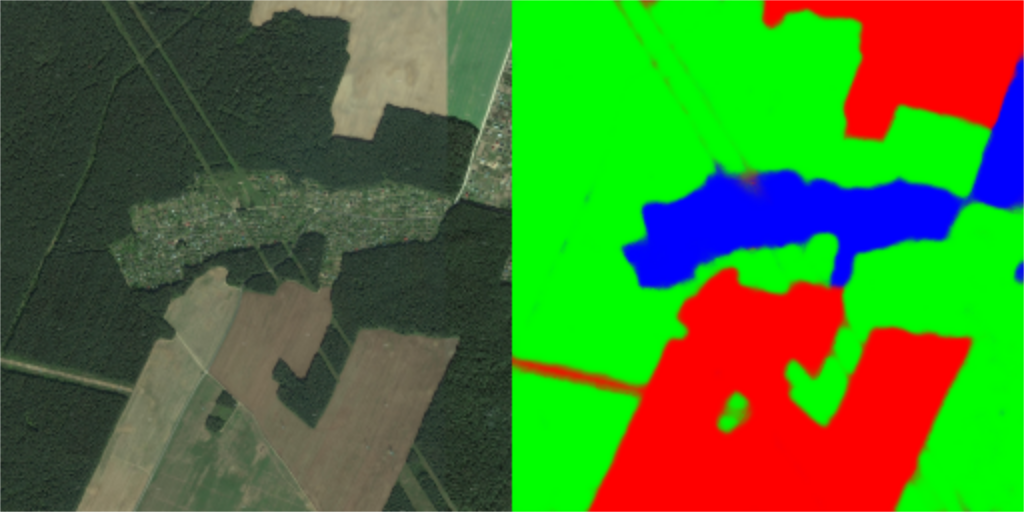
\includegraphics[width=0.8\textwidth]{images/segm_results_yandex.png}
\end{figure}

\addcontentsline{toc}{section}{Метрика IoU}
\section*{Метрика IoU}
Для оценки результатов сегментации, помимо точности, можно посчитать ещё одну
довольно информативную метрику --- \textit{Intersection over Union}
(\textit{IoU}). Она вычисляется для бинарных изображений, т.е. тех, где каждый
пиксель отнесён к одному из двух классов. Поэтому изображения карты вероятностей
нужно сначала обрезать по какому-либо порогу $T$. Т.е. заменить значения меньше
$T$ на $0$, а больше $T$ --- на $1$. Затем два сравниваемых изображения
(истинная маска и результат работы алгоритма) рассматриваются как множества
точек, в которых находятся $1$. Пусть это множества $A$ и $B$ (порядок не
важен). Тогда значение $\Omega$ метрики IoU равно
$$
\Omega = \frac{A \cap B}{A \cup B}
$$
Чем ближе значение $\Omega$ к $1$, тем лучше качество сегментации.
